%
% Documento: Resultados
%

\chapter{Resultados experimentais}
\label{cap:resultados}

Este capítulo apresenta os resultados obtidos na campanha de medições. Todos os percentuais, tempos e valores de RSSI bruto descritos a seguir foram calculados a partir dos dados coletados; nenhum deles foi estimado por cálculo teórico.

O objetivo é discutir o comportamento observado do conjunto formado por YPD-R200, APCA8090 e AD-239 M730, verificar as métricas propostas e destacar as condições que mais afetaram a leitura. Os níveis de RSSI foram preservados apenas como indicador relativo do leitor, pois não houve calibração para dBm.

% Tabelas elaboradas a partir dos dados experimentais coletados.
% Os níveis de RSSI são apresentados na unidade bruta informada pelo módulo.

\newcommand{\TabelaAlcanceDistancia}{%
\begin{table}[htbp]
    \centering
    \caption{Síntese descritiva das medições por distância horizontal.}
    \label{tab:resultado-alcance-distancia}
    \small
    \setlength{\tabcolsep}{7pt}
    \begin{tabular}{cccc}
        \toprule
        \textbf{\shortstack{Distância\\(m)}} &
        \textbf{\shortstack{Detecções\\($n/N$)}} &
        \textbf{\shortstack{Taxa de\\leitura}} &
        \textbf{IC 95\% de Wilson} \\
        \midrule
        0,5 & 15/15 & 100,0\% & 79,6\% a 100,0\% \\
        1,0 & 85/105 & 81,0\% & 72,4\% a 87,3\% \\
        1,5 & 47/60 & 78,3\% & 66,4\% a 86,9\% \\
        2,0 & 67/105 & 63,8\% & 54,3\% a 72,4\% \\
        5,0 & 0/90 & 0,0\% & 0,0\% a 4,1\% \\
        \bottomrule
    \end{tabular}
    \fonte{Elaborado pelo autor a partir dos dados experimentais (2026).}
\end{table}%
}

\newcommand{\TabelaOrientacao}{%
\begin{table}[htbp]
    \centering
    \caption{Síntese descritiva das medições por orientação da etiqueta.}
    \label{tab:resultado-orientacao}
    \small
    \setlength{\tabcolsep}{7pt}
    \begin{tabular}{cccc}
        \toprule
        \textbf{\shortstack{Orientação\\($^\circ$)}} &
        \textbf{\shortstack{Detecções\\($n/N$)}} &
        \textbf{\shortstack{Taxa de\\leitura}} &
        \textbf{IC 95\% de Wilson} \\
        \midrule
        0 & 115/165 & 69,7\% & 62,3\% a 76,2\% \\
        45 & 60/105 & 57,1\% & 47,6\% a 66,2\% \\
        90 & 39/105 & 37,1\% & 28,5\% a 46,7\% \\
        \bottomrule
    \end{tabular}
    \fonte{Elaborado pelo autor a partir dos dados experimentais (2026).}
\end{table}%
}

\newcommand{\TabelaMaterial}{%
\begin{table}[htbp]
    \centering
    \caption{Resultado experimental por material de fixação.}
    \label{tab:resultado-material}
    \small
    \setlength{\tabcolsep}{4pt}
    \begin{tabular}{lcccc}
        \toprule
        \textbf{Material de fixação} &
        \textbf{\shortstack{Detecções\\($n/N$)}} &
        \textbf{\shortstack{Taxa de\\leitura}} &
        \textbf{IC 95\%} &
        \textbf{\shortstack{RSSI bruto\\média $\pm$ DP}} \\
        \midrule
        Papelão & 5/5 & 100,0\% & 56,6\% a 100,0\% & 183,0 $\pm$ 4,5 \\
        Metal direto & 0/5 & 0,0\% & 0,0\% a 43,4\% & Sem leitura \\
        Metal com espaçador & 5/5 & 100,0\% & 56,6\% a 100,0\% & 182,6 $\pm$ 4,2 \\
        \bottomrule
    \end{tabular}
    \fonte{Elaborado pelo autor a partir dos dados experimentais (2026).}
\end{table}%
}

\newcommand{\TabelaPorEtiqueta}{%
\begin{table}[htbp]
    \centering
    \caption{Desempenho por conjunto formado pela etiqueta e pelo suporte no subconjunto com registros individuais.}
    \label{tab:resultado-por-tag}
    \small
    \setlength{\tabcolsep}{4pt}
    \begin{tabular}{lrrrr}
        \toprule
        \textbf{\shortstack{Etiqueta\\e suporte}} &
        \textbf{\shortstack{Distância\\detecções ($n/N$)}} &
        \textbf{\shortstack{Taxa de\\leitura}} &
        \textbf{\shortstack{Orientação\\detecções ($n/N$)}} &
        \textbf{\shortstack{Taxa de\\leitura}} \\
        \midrule
        TAG1 (papelão) & 15/20 & 75,0\% & 13/15 & 86,7\% \\
        TAG2 (madeira) & 17/20 & 85,0\% & 13/15 & 86,7\% \\
        TAG3 (plástico) & 12/20 & 60,0\% & 11/15 & 73,3\% \\
        \bottomrule
    \end{tabular}
    \fonte{Elaborado pelo autor a partir dos dados experimentais (2026).}
\end{table}%
}

\newcommand{\TabelaInventarioRodadas}{%
\begin{table}[htbp]
    \centering
    \caption{Cobertura por rodada no inventário experimental em sala.}
    \label{tab:resultado-inventario-rodadas}
    \small
    \setlength{\tabcolsep}{6pt}
    \begin{tabular}{ccccc}
        \toprule
        \textbf{Rodada} &
        \textbf{\shortstack{Etiquetas\\detectadas}} &
        \textbf{Cobertura} &
        \textbf{\shortstack{Rodada\\completa}} &
        \textbf{\shortstack{Leituras\\externas}} \\
        \midrule
        1 & 4 & 80,0\% & Não & 0 \\
        2 & 4 & 80,0\% & Não & 0 \\
        3 & 4 & 80,0\% & Não & 0 \\
        4 & 4 & 80,0\% & Não & 0 \\
        5 & 3 & 60,0\% & Não & 0 \\
        \bottomrule
    \end{tabular}
    \fonte{Elaborado pelo autor a partir dos dados experimentais (2026).}
\end{table}%
}

\newcommand{\TabelaInventarioResumo}{%
\begin{table}[htbp]
    \centering
    \caption{Resumo do inventário experimental.}
    \label{tab:resultado-inventario}
    \small
    \begin{tabular}{p{6.2cm}r}
        \toprule
        \textbf{Métrica} & \textbf{Valor} \\
        \midrule
        Rodadas analisadas & 5 \\
        Etiquetas presentes por rodada & 5 \\
        Cobertura média & 76,0\% \\
        Desvio-padrão da cobertura & 8,9 pontos percentuais \\
        IC 95\% da cobertura média & 64,9\% a 87,1\% \\
        Faixa de cobertura & 60,0\% a 80,0\% \\
        Taxa de rodadas completas & 0/5 = 0,0\% \\
        IC 95\% da taxa de rodadas completas & 0,0\% a 43,4\% \\
        Leituras externas totais & 0 \\
        Leituras repetidas totais & 54 \\
        Leituras repetidas médias por rodada & 10,8 \\
        Leituras válidas médias por rodada & 14,6 \\
        \bottomrule
    \end{tabular}
    \fonte{Elaborado pelo autor a partir dos dados experimentais (2026).}
\end{table}%
}


\section{Distância horizontal}

A \autoref{tab:resultado-alcance-distancia} mostra que a taxa de leitura foi de 100,0\% a 0,5~m, 73,3\% a 1,0~m, 66,7\% a 1,5~m e 53,3\% a 2,0~m. Os respectivos intervalos de confiança de 95\% foram de 79,6\% a 100,0\%, de 48,0\% a 89,1\%, de 41,7\% a 84,8\% e de 30,1\% a 75,2\%. A tendência observada é de queda com a distância, mas a amplitude dos intervalos evidencia a incerteza decorrente das 15 tentativas por condição.

\TabelaAlcanceDistancia

A \autoref{fig:resultado-alcance-distancia} representa graficamente as taxas e os intervalos da \autoref{tab:resultado-alcance-distancia} nos quatro níveis efetivamente ensaiados.

\begin{figure}[htbp]
    \centering
    \caption{Taxa experimental de leitura em função da distância horizontal; as barras de erro representam o IC 95\% de Wilson.}
    \label{fig:resultado-alcance-distancia}
    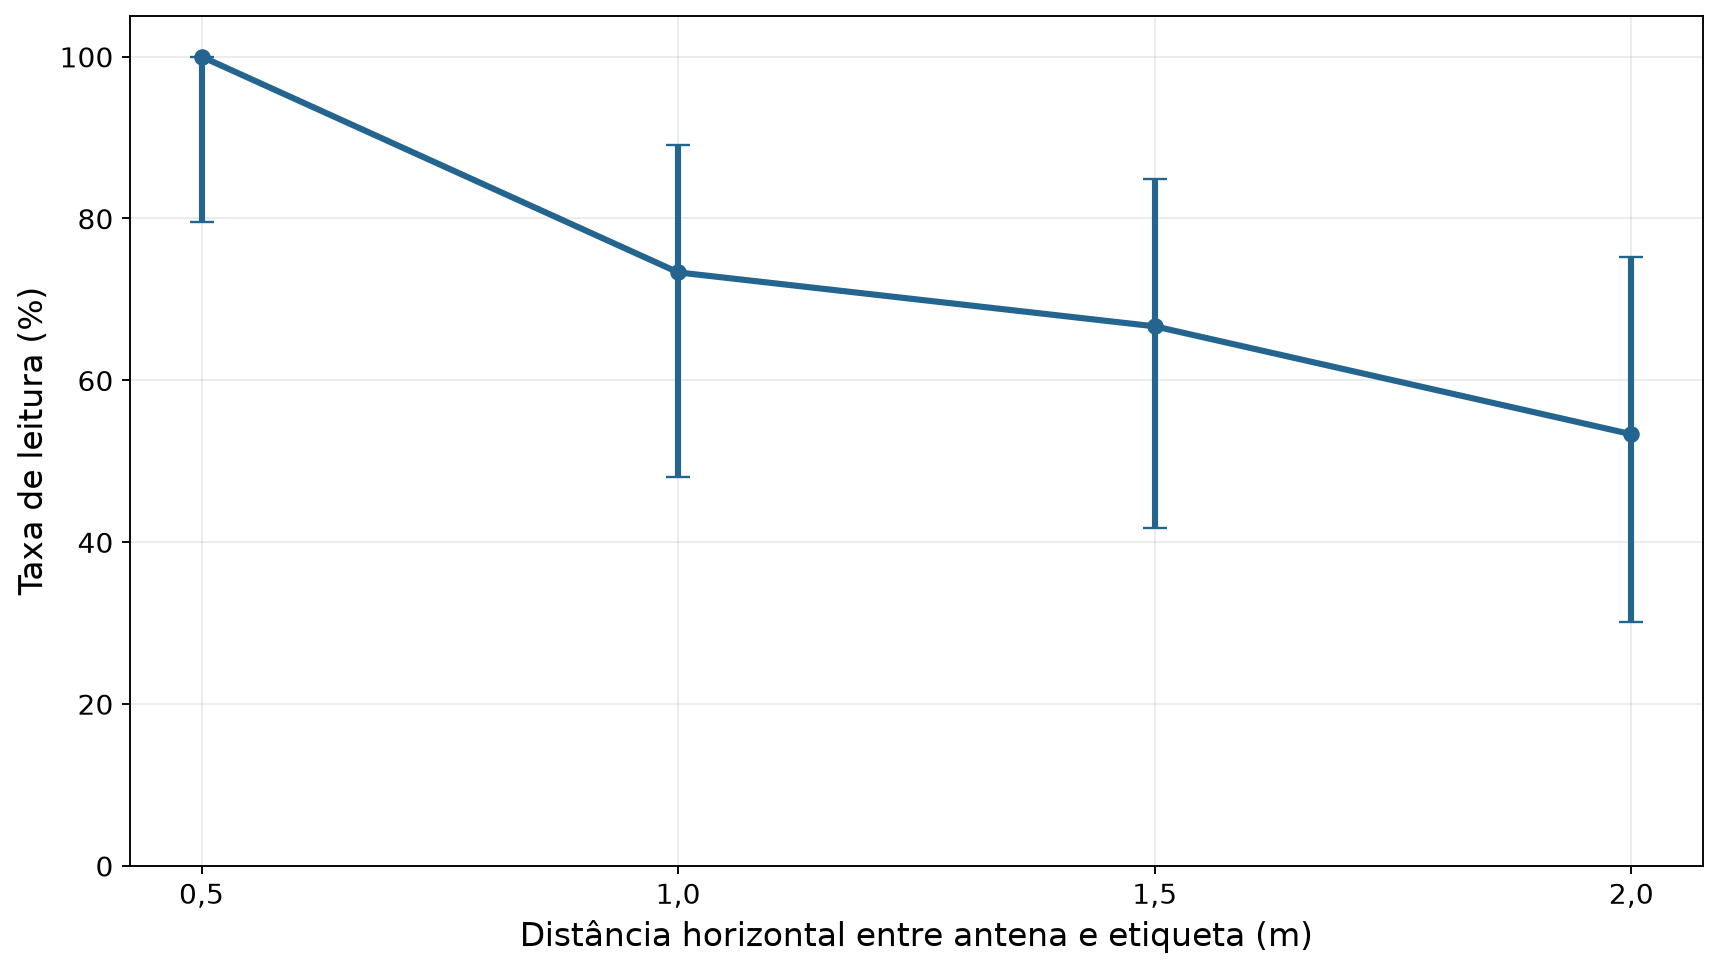
\includegraphics[width=0.82\textwidth]{./04-figuras/resultado_alcance_distancia}
    \fonte{Elaborado pelo autor a partir dos dados experimentais (2026).}
\end{figure}

\FloatBarrier

Adotando 90\% como limiar diagnóstico de repetibilidade por condição, apenas o ponto de 0,5~m atingiu o critério nesta campanha. Como a próxima distância ensaiada foi 1,0~m, os dados não permitem localizar com precisão o limite entre esses dois pontos. Esse limiar não constitui aceitação operacional para o inventário, pois detectar 90\% das tentativas ou dos bens ainda deixa omissões. Para uma passagem pela sala, o requisito adotado é identificar todos os EPCs esperados na mesma rodada.

Na \autoref{tab:resultado-alcance-distancia}, o tempo médio até a primeira leitura, calculado somente entre tentativas com detecção, cresce com a distância: $0{,}020 \pm 0{,}003$~s a 0,5~m, $0{,}206 \pm 0{,}338$~s a 1,0~m, $0{,}596 \pm 0{,}726$~s a 1,5~m e $0{,}773 \pm 0{,}846$~s a 2,0~m. A dispersão elevada nos três últimos pontos mostra que a média temporal deve ser interpretada com cautela; tentativas sem detecção não entram nesse cálculo e já são representadas pela taxa de sucesso. As médias de RSSI bruto também não variaram de forma monotônica com a distância. Como o RSSI não foi calibrado e o multipercurso integrou o cenário realista sem ser medido separadamente, esses valores descrevem apenas o comportamento relativo observado; eles não podem ser convertidos para potência em dBm nem utilizados para isolar causalmente os mecanismos de propagação. Além disso, TAG1, TAG2 e TAG3 permaneceram associadas, respectivamente, a papelão, madeira e plástico. Como os mesmos três conjuntos foram usados em todas as distâncias, a comparação agregada entre distâncias conserva a composição do painel, mas uma diferença individual não pode ser atribuída somente à etiqueta.

\section{Orientação}

A \autoref{tab:resultado-orientacao} mostra que o conjunto obteve 93,3\% de leitura em 0$^\circ$, 86,7\% em 45$^\circ$ e 66,7\% em 90$^\circ$, sempre a 1,5~m. Os intervalos de confiança de 95\% foram, respectivamente, de 70,2\% a 98,8\%, de 62,1\% a 96,3\% e de 41,7\% a 84,8\%. A tendência monotônica é compatível com a perda de acoplamento por desalinhamento entre polarizações lineares. Em um cenário institucional fechado, o multipercurso faz parte das condições normais de operação. Como os intervalos se sobrepõem e esse efeito não foi medido separadamente, os dados não permitem atribuir toda a diferença exclusivamente ao ângulo. Os três conjuntos formados por etiqueta e suporte aparecem em todos os ângulos, mas a associação fixa entre exemplar e suporte permanece como fator de confusão na análise individual.

\TabelaOrientacao

A \autoref{fig:resultado-orientacao} permite comparar visualmente a tendência entre os três ângulos, preservando a amplitude dos intervalos de confiança.

\begin{figure}[htbp]
    \centering
    \caption{Taxa experimental de leitura nas orientações testadas a 1,5~m; as barras de erro representam o IC 95\% de Wilson.}
    \label{fig:resultado-orientacao}
    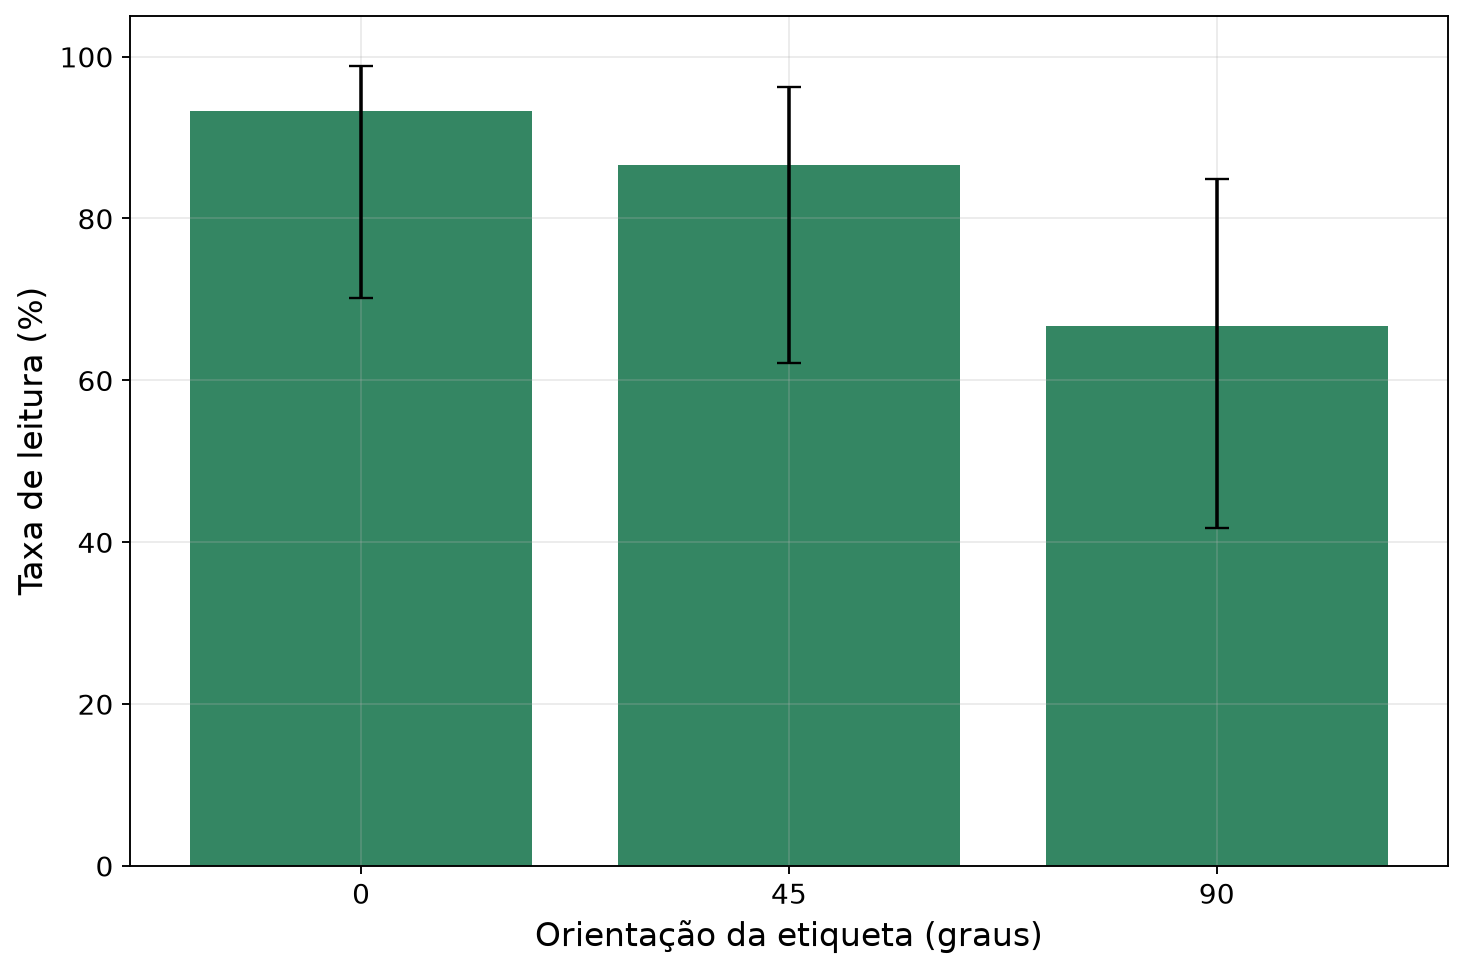
\includegraphics[width=0.70\textwidth]{./04-figuras/resultado_orientacao}
    \fonte{Elaborado pelo autor a partir dos dados experimentais (2026).}
\end{figure}

A análise complementar por conjunto formado por etiqueta e suporte é apresentada na \autoref{tab:resultado-por-tag}.

\TabelaPorEtiqueta

\FloatBarrier

A \autoref{tab:resultado-por-tag} apresenta uma verificação complementar por conjunto. No ensaio de distância, TAG1 com papelão, TAG2 com madeira e TAG3 com plástico obtiveram, respectivamente, 75,0\%, 85,0\% e 60,0\%; no ensaio de orientação, as taxas foram 86,7\%, 86,7\% e 73,3\%. Essa variação descreve os conjuntos efetivamente usados, mas não permite concluir que uma etiqueta, madeira ou plástico foi responsável pela diferença, pois exemplar e suporte não foram variados independentemente.

\section{Ensaio complementar com uma etiqueta isolada}

A \autoref{tab:resultado-ensaio-uma-tag} reúne o ensaio complementar com uma única etiqueta na zona de leitura. Em 1,0~m, as taxas foram 100,0\%, 86,7\% e 60,0\% para 0$^\circ$, 45$^\circ$ e 90$^\circ$. Em 2,0~m, os valores caíram para 90,0\%, 70,0\% e 36,7\%. Em 5,0~m, não houve detecção nas 30 tentativas de cada orientação. Os intervalos de Wilson permanecem apresentados porque, mesmo com 30 tentativas por combinação, as proporções não constituem valores exatos da população.

\TabelaEnsaioUmaTag

O bloco complementar evidencia uma interação prática entre distância e orientação: o alinhamento de 0$^\circ$ preservou desempenho elevado em 1,0 e 2,0~m, enquanto o desalinhamento reduziu a repetibilidade, e 5,0~m ficou fora do alcance útil nas condições observadas. Como essas falhas ocorreram com apenas uma etiqueta respondendo, colisões entre tags não são necessárias para explicar parte das omissões. O multipercurso, o limiar de energização da tag, a polarização, a aquisição serial e outras fontes de variabilidade ainda podem atuar. O ensaio não quantifica a contribuição de colisões no inventário; isso exigiria comparar, na mesma geometria e sob o mesmo protocolo, cada etiqueta isolada e as mesmas etiquetas presentes simultaneamente.

Os registros desse bloco foram preservados apenas como contagens consolidadas. Eles não contêm RSSI, tempos individuais, ordem das tentativas ou diagnósticos seriais suficientes para combinação com os demais ensaios. Por essa razão, a matriz complementa a interpretação de distância e orientação, mas não altera as estatísticas das tabelas anteriores.

\FloatBarrier

\section{Material de fixação}

Na \autoref{tab:resultado-material}, papelão e metal com espaçador plástico de 10~mm apresentaram 100,0\% de leitura, enquanto o metal direto resultou em 0,0\%. Como houve apenas cinco tentativas e um único exemplar de tag por condição, os intervalos de 95\% ainda são amplos: de 56,6\% a 100,0\% nos dois casos de sucesso integral e de 0,0\% a 43,4\% no metal direto.

\TabelaMaterial

A \autoref{fig:resultado-material} destaca o contraste entre o contato metálico direto e as duas condições nas quais houve detecção.

\begin{figure}[htbp]
    \centering
    \caption{Taxa experimental de leitura para os materiais de fixação testados; as barras de erro representam o IC 95\% de Wilson.}
    \label{fig:resultado-material}
    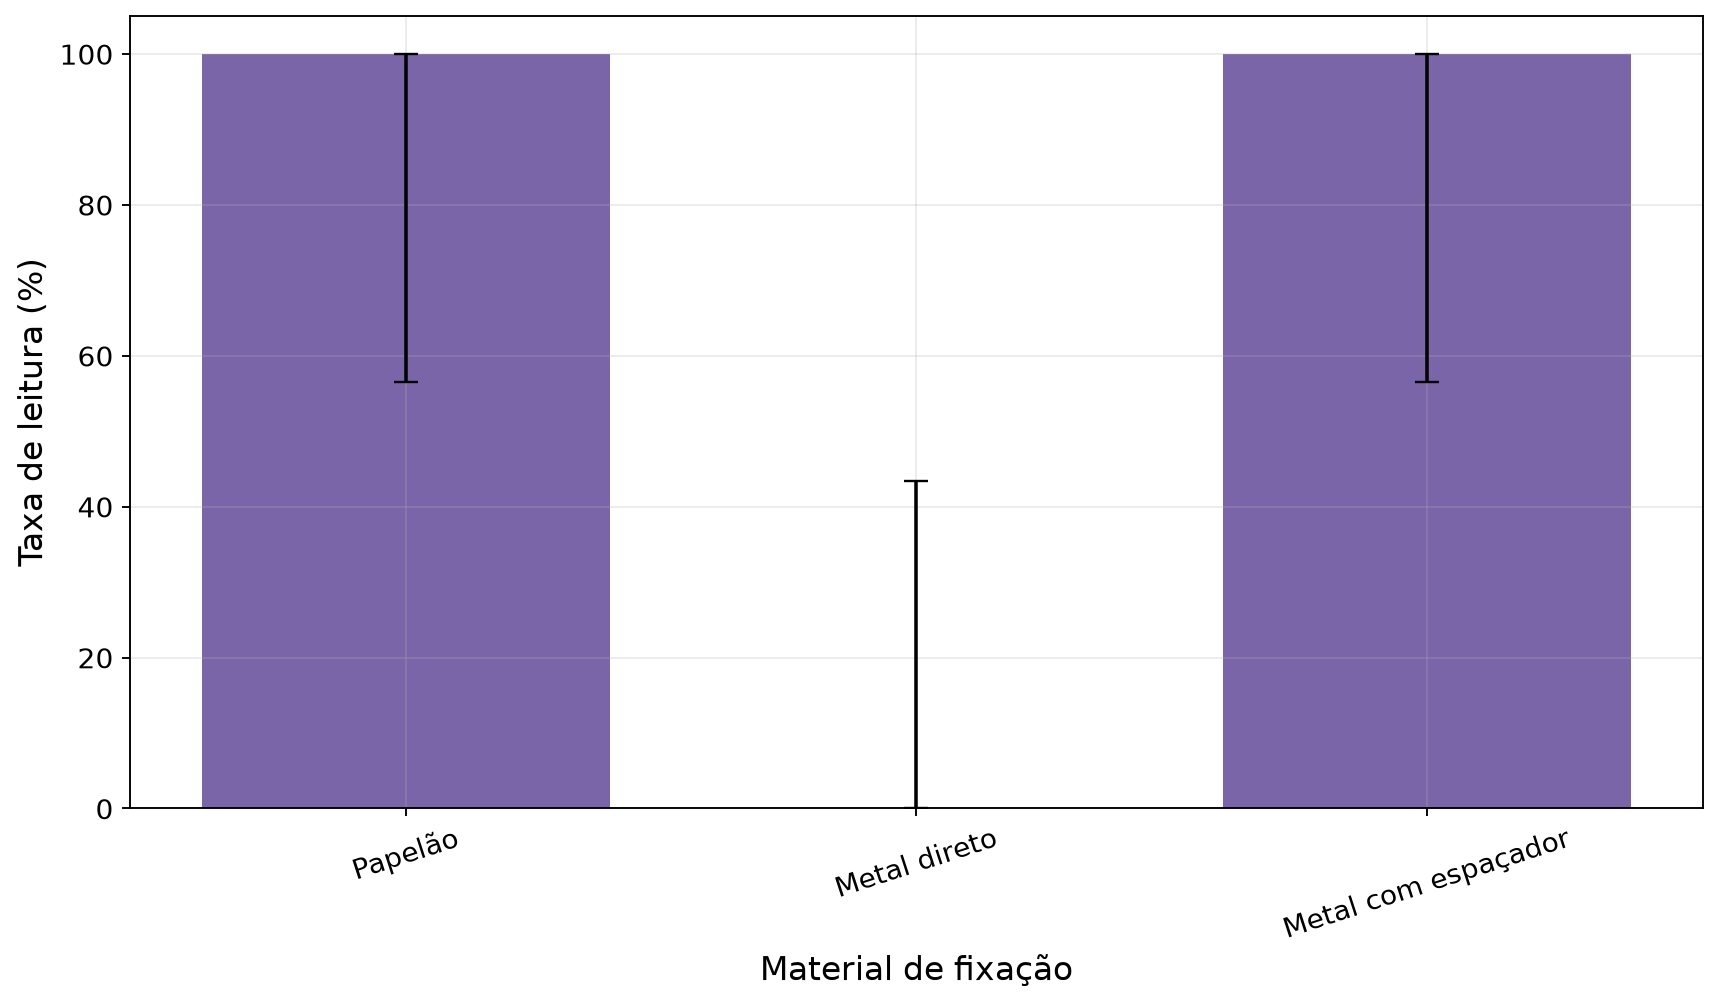
\includegraphics[width=0.82\textwidth]{./04-figuras/resultado_material}
    \fonte{Elaborado pelo autor a partir dos dados experimentais (2026).}
\end{figure}

\FloatBarrier

O espaçador de 10~mm recuperou a leitura nas cinco tentativas realizadas, fornecendo evidência favorável à separação física nessa montagem. O resultado não permite definir 10~mm como espessura ótima nem substituir a validação com etiquetas próprias para metal. Para a prática patrimonial, ele indica que bens metálicos exigem etiqueta adequada ou suporte auxiliar previamente testado.

\section{Inventário em sala}

O inventário em sala apresentou cobertura de 80\% nas rodadas 1 a 4 e de 60\% na rodada 5, com média de 76,0\%, desvio-padrão de 8,9 pontos percentuais e IC 95\% da média de 64,9\% a 87,1\%. Nenhuma das cinco rodadas foi completa. Portanto, a taxa observada de inventários completos foi de 0,0\%, com IC 95\% de Wilson de 0,0\% a 43,4\%. O intervalo da cobertura média informa quantas etiquetas foram encontradas, em média, e não a chance de concluir a conferência. A taxa de rodadas completas é a métrica diretamente relacionada ao requisito de identificar todos os bens em uma passagem. As tags foram avaliadas ao longo de um percurso curto padronizado em laboratório fechado de aproximadamente 50~m$^2$, configuração compatível com uma operação cotidiana de inventário institucional. Como dimensões lineares, coordenadas individuais e trajeto exato não foram registrados, não é possível reproduzir integralmente a geometria, mas essa ausência não descaracteriza a avaliação do desempenho agregado no cenário de uso. A \autoref{tab:resultado-inventario-rodadas} detalha cada rodada e a \autoref{tab:resultado-inventario} reúne os indicadores consolidados.

\TabelaInventarioRodadas
\TabelaInventarioResumo

A \autoref{fig:resultado-inventario} mostra a estabilidade das quatro primeiras rodadas e a redução observada na quinta.

\begin{figure}[htbp]
    \centering
    \caption{Cobertura por rodada no inventário experimental em sala.}
    \label{fig:resultado-inventario}
    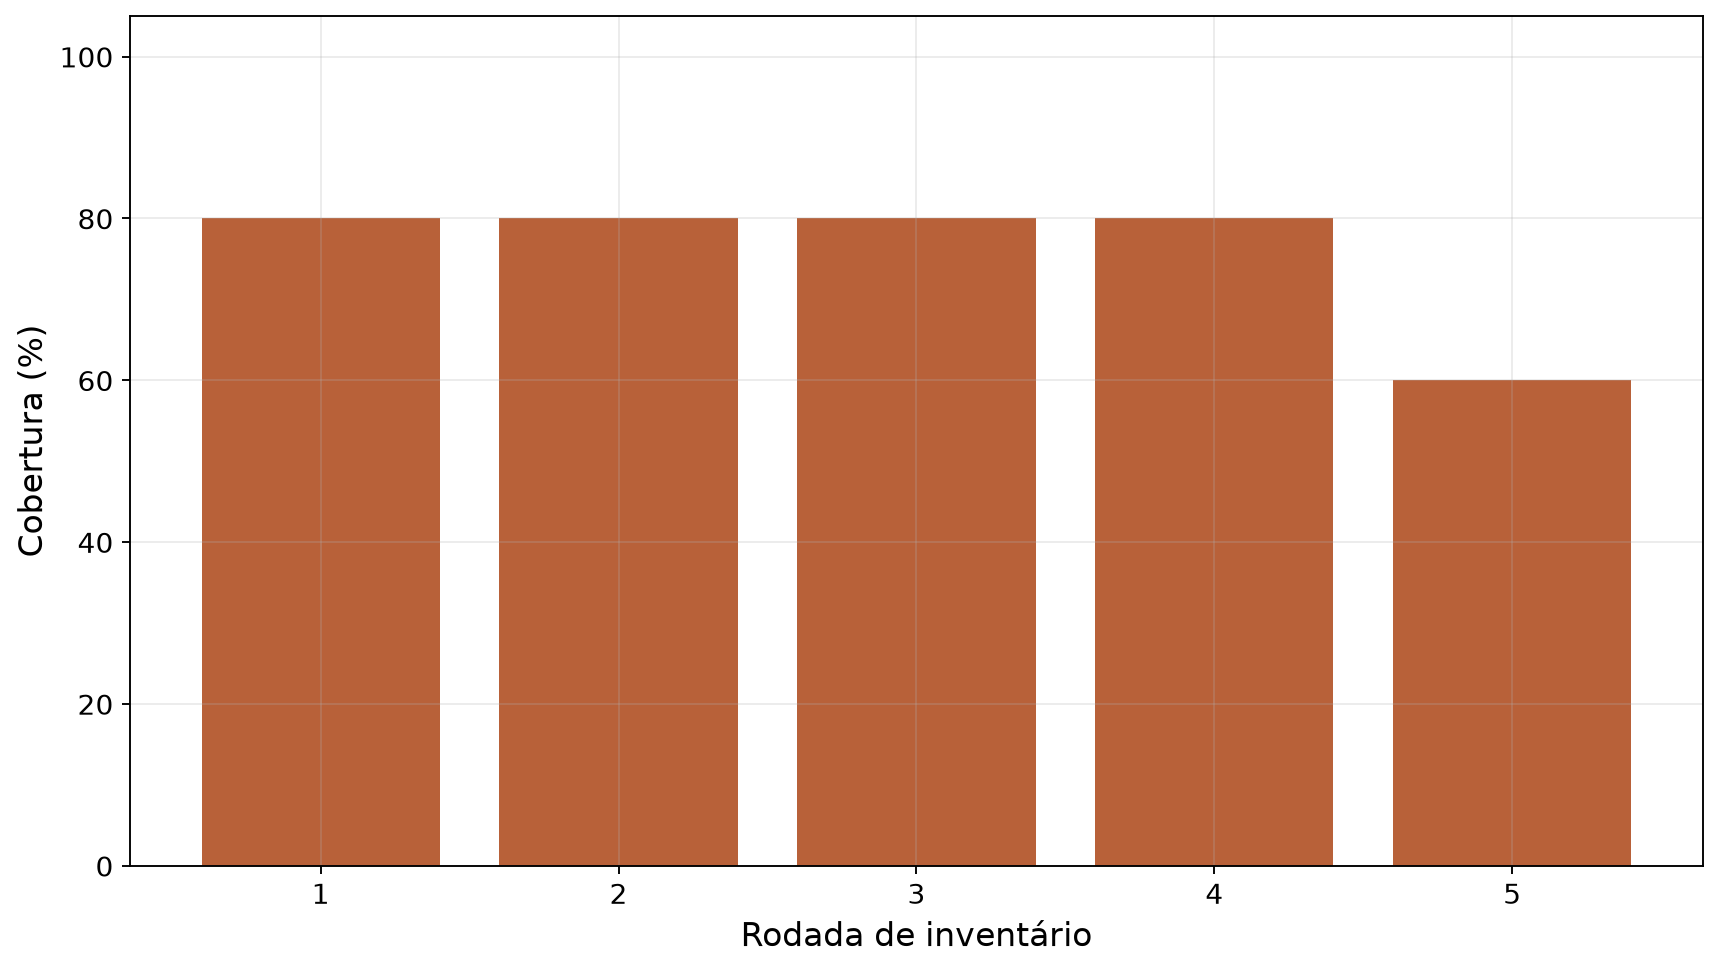
\includegraphics[width=0.82\textwidth]{./04-figuras/resultado_inventario}
    \fonte{Elaborado pelo autor a partir dos dados experimentais (2026).}
\end{figure}

\FloatBarrier

A ausência de rodadas completas mostra que, em ambiente comum e com apenas uma antena, a cobertura média não basta para garantir inventário completo. O IC da taxa de rodadas completas é amplo devido às cinco rodadas e não demonstra que a probabilidade real seja exatamente zero. Ainda assim, nenhuma execução satisfez o requisito, de modo que os dados não sustentam o uso da configuração atual como referência operacional. Foram registrados 73 quadros válidos: 19 correspondem às detecções distintas somadas entre as rodadas e 54 foram repetições de EPC já visto na mesma janela. Não houve leitura externa nas cinco rodadas oficiais. O firmware deduplicou esses quadros antes de calcular a cobertura, conforme definido na metodologia. A presença aproximada de cinco pessoas e quatro objetos metálicos próximos caracteriza uma condição usual de laboratório e aumenta a representatividade prática do ensaio. Como esses elementos não foram variados independentemente, os resultados descrevem o desempenho do conjunto no cenário completo, e não o efeito isolado de cada componente ambiental.

As cinco etiquetas formavam a etapa inicial de uma progressão planejada até aproximadamente 50 unidades. Como a cobertura integral não ocorreu sequer nessa etapa, aumentar a população não permitiria corrigir a limitação física já observada. O escalonamento foi interrompido para priorizar a revisão de antena, etiquetas, geometria e configuração do leitor. Essa decisão não estabelece que cinco seja a capacidade máxima do YPD-R200; a capacidade de inventário do protocolo não foi medida, pois o critério mínimo de desempenho da montagem falhou antes do teste de escala.

\section{Integridade da aquisição}

Após as medições, verificou-se que a alternância entre a fonte externa de 5~V/1~A e a alimentação pela conexão USB do Arduino não produziu alteração relevante nos resultados obtidos.

Os registros diagnósticos coletados permitem avaliar a aquisição sem atribuir automaticamente toda falha à interface de RF. Nas 693 consultas dos ensaios principais de distância, orientação e material, ocorreram 21 quadros inválidos (3,0\%), 9 \textit{timeouts} (1,3\%) e nenhum erro de comando. No inventário, foram 251 consultas, 5 quadros inválidos (2,0\%), 2 \textit{timeouts} (0,8\%) e nenhum estouro da tabela de EPCs. O ensaio complementar de uma etiqueta não integra essas contagens, pois seus registros foram preservados apenas de forma agregada. Esses percentuais são diagnósticos do programa, e não uma taxa de erro de enquadramento da UART: sem analisador lógico, não é possível distinguir completamente corrupção em \texttt{SoftwareSerial}, resposta malformada do módulo e efeitos do enlace entre leitor e tag.

\section{Síntese da discussão}

Os resultados sustentam as três tendências principais da hipótese: a repetibilidade caiu com a distância, o contato direto com metal impediu a detecção da etiqueta convencional e a taxa diminuiu com o aumento do desalinhamento angular. O ensaio de etiqueta isolada mostra que existem falhas sem disputa simultânea entre tags, de modo que colisão não pode ser tratada como explicação exclusiva para o inventário incompleto. A campanha não separou estatisticamente polarização, multipercurso, suporte, exemplar, serial e anticolisão. Os dados também mostram que o inventário com cinco tags não fechou nenhuma janela, reforçando a necessidade de acumular EPCs únicos, registrar omissões e melhorar a configuração física antes de aumentar a escala.

Em termos de escolha de antena, a APCA8090 linear permitiu estabelecer uma linha de base experimental de baixo custo, mas a configuração não atingiu o requisito operacional. Para tratar diretamente a sensibilidade à orientação, a comparação futura prioritária é com polarização circular ou diversidade de polarização. Uma antena omnidirecional constitui hipótese separada para ampliar a cobertura azimutal e reduzir o esforço de apontamento; ela não corrige por si só o desalinhamento de polarização e pode elevar leituras externas e multipercurso. Bens metálicos também exigem comparar o espaçador com etiquetas próprias para metal.

\section{Requisitos derivados para evolução do protótipo}

Os requisitos da \autoref{tab:requisitos-evolucao} são derivados da campanha. A coluna relativa ao ponto fixo apresenta especificações para trabalho futuro, e não resultados experimentais, pois não houve ensaio de passagem em portal ou zona fixa.

\begin{table}[H]
    \centering
    \caption{Requisitos derivados dos resultados para os cenários portátil e fixo.}
    \label{tab:requisitos-evolucao}
    \footnotesize
    \begin{tabularx}{\textwidth}{p{3.0cm}X X}
        \toprule
        \textbf{Aspecto} & \textbf{Leitor portátil} & \textbf{Ponto fixo} \\
        \midrule
        Zona de leitura & Procedimento deve aproximar a antena das tags e exigir cobertura integral por passagem; 90\% por condição é insuficiente para aceitação. & Cobertura deve ser confinada para reduzir leituras de áreas adjacentes e validada na geometria real da passagem. \\
        Antena e etiquetas & Comparar a APCA8090 com polarização circular ou diversa, avaliar cobertura azimutal e usar tags próprias para metal quando necessário. & Preferir cobertura controlada; inferência de direção exige duas zonas, duas antenas ou sensor auxiliar. \\
        Eletrônica & Usar UART de hardware, confirmar adequação de nível lógico e dimensionar alimentação para o pico do leitor. & Registrar canal/região, potência efetiva e estabilidade em operação prolongada. \\
        Software & Persistir EPC, instante, ambiente e estado da janela; deduplicar antes de calcular cobertura. & Correlacionar eventos por zona e tempo, sem classificar presença isolada como entrada ou saída. \\
        Validação & Após melhorar a configuração, exigir rodadas completas com cinco tags e somente então ampliar gradualmente a população até aproximadamente 50, em mais sessões e ambientes. & Medir leituras externas, omissões e falsos eventos em percursos nos dois sentidos. \\
        \bottomrule
    \end{tabularx}
    \fonte{Elaborado pelo autor a partir dos resultados da campanha (2026).}
\end{table}
